
\section{shelves and streams}


\subsection{shallow shelf aprx (SSA)}

\begin{frame}{shallow shelf approximation (SSA) stress balance}
  
SSA model applies very well to \alert{ice shelves}
\begin{itemize}
\item \dots for parts away from grounding lines
\item \dots and away from calving fronts
\end{itemize}
\end{frame}


\begin{frame}{shallow shelf approximation (SSA) stress balance 2}

SSA also applies reasonably well to \alert{ice streams}
\begin{itemize}
\item \dots with modest bed topography
\item \dots and weak bed strength
\item \dots but not so good near shear margins \& grounding lines
\item energy conservation (= ice temperature and basal melt) is a major aspect of ice stream flow, but not addressed here
\end{itemize}

\begin{center}
  \includegraphics[width=0.5\textwidth]{siple}

\tiny RADARSAT-derived surface velocity for Siple Coast ice streams, Antarctica 
\end{center}
\end{frame}


\begin{frame}{what is, \emph{and is not}, an ice stream?}

\begin{columns}
\begin{column}{0.6\textwidth}
\begin{itemize}
\item ice streams 
  \small
  \begin{itemize}
  \item[$\circ$] slide ($100$ to $1000 \,\text{m}\,\text{a}^{-1}$)
  \item[$\circ$] have concentration of vertical shear in a thin layer near base
  \item[$\circ$] \emph{liquid water} at bed has critical role 
  \end{itemize}
  \normalsize
\item ``outlet glaciers''
  \begin{itemize}
  \item[$\circ$] have fast surface speed (up to $10 \,\text{km}\,\text{a}^{-1}$)
  \item[$\circ$] uncertain how much is true sliding
  \item[$\circ$] substantial vertical shear ``up'' in the ice column
  \item[$\circ$] not-at-all flat bed topography
  \item[$\circ$] soft, temperate ice plays a role
  \end{itemize} 
\item therefore \alert{few simplifying assumptions are appropriate for outlet glaciers}
\end{itemize}
\end{column}

\begin{column}{0.4\textwidth}
\includegraphics[width=1.0\textwidth]{streamisbrae}

\bigskip
\scriptsize 
Cross sections of Jakobshavns Isbrae (\textbf{a}) and
Whillans Ice Stream (\textbf{b}).  Plotted
without vertical exaggeration.  (\tiny Figure 1 in Truffer and Echelmeyer (2003), \emph{Of isbrae and ice streams}\scriptsize)
\end{column}
\end{columns}
\end{frame}


\begin{frame}{SSA stress balance equation}

\begin{itemize}
\item only plane flow case (``flow line'') in these lectures
\item the stress balance equation which determines velocity:
\begin{empheq}[box=\fbox]{equation}
  \left({\color{red}2 B H |u_x|^{1/n - 1} u_x}\right)_x - {\color{blue}C|u|^{m-1}u} = \rho g H h_x \label{ssa}
\end{empheq}
\item the {\color{red} red term} inside parentheses is the vertically-integrated ``longitudinal'' or ``membrane'' stress
\item the {\color{blue} blue term} is basal resistance; $C=0$ in an ice shelf
\item the right-hand side is  driving stress; see \emph{next slide}
\item \emph{how to think about this equation}?
\item \emph{how do you solve it numerically}?
\end{itemize}
\end{frame}


\begin{frame}{flotation criterion and grounding line}

\begin{itemize}
\item the inequality ``$\rho H < - \rho_w b$'' is the \alert{flotation criterion}
\item at the grounding line $x=x_g$ the inequality switches
\item driving stress:
  \begin{itemize}
  \item[$\circ$] on the grounded side $\rho H > - \rho_w b$, so
  	$$\rho g H h_x = \rho g H (H_x + b_x)$$
  \item[$\circ$] on the floating side $\rho H < - \rho_w b$, so $h = (1-\rho/\rho_w) H$, and so
  	$$\rho g H h_x = \rho(1-\rho/\rho_w) g H H_x$$
  \end{itemize}

\vspace{5mm}
\item best numerical models for moving grounding lines still an open question (e.g.~MISMIP and all that)
\end{itemize}
\end{frame}


\begin{frame}{from stream to shelf across grounding line}
\label{slide:streamtoshelf}

\begin{align*}
  u = u_0 & \qquad \text{ at } x = 0 \\
  \left.\begin{array}{r}
  \left(2 B H |u_x|^{1/n - 1} u_x\right)_x - C|u|^{m-1}u = \rho g H h_x \\
  h = H + b
  \end{array}\right\}& \qquad \text{ on } 0 < x < x_g \\
  \left.\begin{array}{r}
  \left(2 B H |u_x|^{1/n - 1} u_x\right)_x + 0 = \rho g H h_x \\
  h = (1-\rho/\rho_w) H
  \end{array}\right\}& \qquad \text{ on } x_g < x < x_c \\
  2 B H |u_x|^{1/n - 1} u_x = \frac{1}{2}\rho (1-\rho/\rho_w) g H^2 & \qquad \text{ at } x = x_c
\end{align*}

\bigskip
\begin{center}
  \includegraphics[width=0.75\textwidth]{flowline}
\end{center}
\end{frame}


\subsection{exact shelf solution}

\begin{frame}{exact velocity and thickness for steady ice shelf}

\begin{itemize}
\item limited goal here: describe a steady state, 1D ice shelf
\item there is this nice \alert{by-hand} result: the thickness and velocity in the ice shelf can be completely determined in terms of the 
  \begin{itemize}
  \item[$\circ$] ice thickness $H_g$ at the grounding line and
  \item[$\circ$] ice velocity $u_g$ at the grounding line
  \end{itemize}
\item derived by van der Veen (1983)
\item shown on next slide
\item we will use this to
  \begin{itemize}
  \item[$\circ$] understand the SSA better
  \item[$\circ$] verify a numerical SSA code
  \end{itemize}
\end{itemize}
\end{frame}


\begin{frame}{exact velocity and thickness for steady ice shelf 2}

\small see \texttt{testshelf.m}:
\bigskip

\begin{columns}
\begin{column}{0.5\textwidth}
  \includegraphics[width=1.0\textwidth]{steadyshelfprofile}

\begin{center}
surface and base elevation (m)
\end{center}
\end{column}
\begin{column}{0.5\textwidth}
  \includegraphics[width=1.0\textwidth]{steadyshelfvelocity}

\begin{center}
velocity (m/a)
\end{center}
\end{column}
\end{columns}

\vspace{10mm}
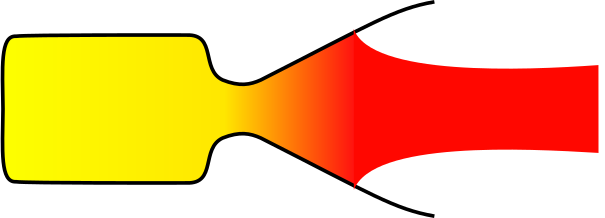
\includegraphics[width=0.2\textwidth]{Rocket_nozzle_expansion}
\end{frame}


\subsection{numerical SSA}

\begin{frame}{numerically solving the SSA stress balance}

\begin{itemize}
\item now we fix ice thickness $H(x)$ and find the velocity numerically
\item the stress balance is a nonlinear equation in the velocity:
  $$\left(2 B H |u_x|^{1/n - 1} u_x\right)_x - C|u|^{m-1}u = \rho g H h_x$$
\item nonlinear so \alert{iteration is needed}
\end{itemize}
\end{frame}


\begin{frame}{Picard iteration}

\begin{itemize}
\item coefficient ${\color{red} \bar \nu} = B |u_x|^{1/n-1}$ is the ``effective viscosity'':
   $$\left(2 \,{\color{red} \bar \nu}\, H u_x\right)_x - C |u|^{m-1} u = \rho g H h_x$$
\item \emph{simplest iteration idea}: use initial velocity estimate to get effective viscosity estimate, then solve for new velocity, and repeat until things stop changing
  \begin{itemize}
  \item[$\circ$] this is ``Picard'' iteration
  \item[$\circ$] Newton iteration is a superior alternative
  \end{itemize}
\item the iteration in formulas:
  \begin{enumerate}
  \item previous iterate $u^{(k-1)}$
  \item define $W^{(k-1)} = 2 \bar \nu H = 2 B |u^{(k-1)}_x|^{1/n-1} H$
  \item solve for current iterate (unknown) $u^{(k)}$:
     $$\left(W^{(k-1)} u^{(k)}_x\right)_x - C |u^{(k-1)}|^{m-1} u^{(k)} = \rho g H h_x$$
  \item repeat at 1
  \end{enumerate}
\end{itemize}
\end{frame}


\begin{frame}{where do you get an initial velocity $u^{(0)}$?}

\begin{itemize}
\item \emph{for floating ice}, an initial guess assumes uniform strain rate:
   $$u^{(0)}(x) = \gamma (x-x_g) + u_g$$
where $\gamma$ is the value of $u_x$ from calving front stress imbalance
\item \emph{for grounded ice}, an initial guess assumes ice is held by basal resistance only:
   $$u^{(0)}(x) = \left(-C^{-1} \rho g H h_x\right)^{1/m}$$
\end{itemize}
\end{frame}


\begin{frame}{a linear problem at each iteration}
\begin{itemize}
\item abstract the problem:
   $$\left(W(x)\, u_x\right)_x - \alpha(x)\, u = \beta(x)$$
on $0 < x < L$, with boundary conditions
   $$u(0) = V, \qquad  u_x(L) = \gamma$$
\item an \emph{linear}, elliptic PDE boundary value problem
\item $W(x)$, $\alpha(x)$, $\beta(x)$ are known functions in the SSA context:
  \begin{itemize}
  \item[$\circ$] both $W(x)$ and $\alpha(x)$ come from previous iteration
  \item[$\circ$] $\beta(x)$ is driving stress
  \end{itemize}
\end{itemize}
\end{frame}


\begin{frame}{numerics of the linear problem}

\begin{itemize}
\item equally-spaced grid $x_1,x_2,\dots,x_{J+1}$
  \begin{itemize}
  \item[$\circ$] $x_1 = x_g$ and $x_{J+1} = x_c$ are endpoints
  \end{itemize}
\item the finite difference approximation to the linear PDE is:
$$\frac{W_{j+1/2} (u_{j+1} - u_j) - W_{j-1/2} (u_{j} - u_{j-1})}{\Delta x^2} - \alpha_j u_j \stackrel{\ast}{=} \beta_j$$
\item so $W(x)$ is needed on the staggered grid
\item left-hand boundary condition: $u_1 = V$ given
\item right-hand boundary condition is $u_x(L)=\gamma$
\item to put right-hand b.c.~into system:
  \begin{itemize}
  \item[$\circ$] introduce notional point $x_{J+2}$
  \item[$\circ$]
    $$\frac{u_{J+2} - u_J}{2 \Delta x} = \gamma$$
  \item[$\circ$] using equation $\ast$ in $j=J+1$ case, eliminate $u_{J+2}$ variable by-hand before solving system
  \end{itemize}
\end{itemize}
\end{frame}


\begin{frame}{numerics of the linear problem 2}

\small
\begin{itemize}
\item thus discretized stress balance has form  \, $A \mathbf{x} = \mathbf{b}$\, :
$$
\begin{bmatrix}
1 &  &  &  &  \\
W_{3/2} & A_{22} & W_{5/2} &  &  \\
 & W_{5/2} & A_{33} &  &  \\
 &  & \ddots & \ddots &  \\
 &  & W_{J-1/2} & A_{JJ} & W_{J+1/2} \\
 &  &  & A_{J+1,J} & A_{J+1,J+1} \\
\end{bmatrix}\,
\begin{bmatrix}
u_1 \\ u_2 \\ u_3 \\ \vdots \\ u_J \\ u_{J+1}
\end{bmatrix}
=
\begin{bmatrix}
0 \\ \beta_2 \Delta x^2 \\ \beta_3 \Delta x^2 \\ \vdots \\ \beta_J \Delta x^2 \\ b_{J+1}
\end{bmatrix}
$$
\item with specific formulas on diagonal ($A_{jj}$) and in the last equation
  \begin{itemize}
  \small
  \item[$\circ$] see printed notes
  \end{itemize}
\item this is a \emph{tridiagonal} system
\item hand the system to a linear algebra black box
\end{itemize}
\end{frame}


\begin{frame}{solver for the linear problem}

\minput{flowline}

\vspace{-4mm}
\begin{itemize}
\item solves
   $$\left(W(x)\, u_x\right)_x - \alpha(x)\, u = \beta(x)$$
\end{itemize}
\end{frame}


\begin{frame}{testing the linear PDE solver}

\begin{itemize}
\item before proceeding to solve nonlinear SSA problem, we can test the ``abstracted'' code \texttt{flowline.m}
\item test by ``manufacturing'' solutions
  \begin{itemize}
  \item[$\circ$] see \texttt{testflowline.m}; not shown
  \end{itemize}
\item results:  converges at optimal rate $O(\Delta x^2)$
\end{itemize}
\end{frame}


\begin{frame}{numerical: SSA}

\vspace{-3mm}
\minputtiny{ssaflowline}

\vspace{-5mm}
\small
\begin{itemize}
\item implements the Picard iteration
\item calls the linear solver \texttt{flowline.m} at each iteration
\end{itemize}
\end{frame}


\begin{frame}[fragile]
  \frametitle{\emph{numerical} velocity for a steady ice shelf}

\begin{itemize}
\item left: exact (red curve) and numerical (green circles) velocity
  \begin{itemize}
  \item[$\circ$] for very coarse 8 km grid
  \item[$\circ$] blue is initial velocity iterate
  \end{itemize}
\item right: convergence analysis of \texttt{ssaflowline.m}
  \begin{itemize}
  \item[$\circ$] error = max(numerical - exact), over various grids
  \end{itemize}
\end{itemize}

\begin{columns}
\begin{column}{0.5\textwidth}
  \includegraphics[width=1.0\textwidth]{ssavel8km}
\end{column}
\begin{column}{0.5\textwidth}
  \includegraphics[width=1.0\textwidth]{shelfconv}
\end{column}
\end{columns}

\end{frame}



\subsection{real ice shelves}

\begin{frame}{realistic ice shelf modeling}

\begin{itemize}
\item flow lines are never very realistic
\item you can add ``side drag''
  \begin{itemize}
  \item[$\circ$] I don't know how to parameterize it
  \end{itemize}
\item also, ice shelves have surprises:
  \begin{itemize}
  \item[$\circ$] high basal melt near grounding lines
  \item[$\circ$] ``reverse bed slope'' instability
  \item[$\circ$] marine ice can freeze-on at bottom (below)
  \end{itemize}
\end{itemize}

\medskip
\begin{center}
  \includegraphics[width=0.5\textwidth]{marineice}
  
  \medskip
  \tiny Filchner-Ronne ice shelf; from Grosfeld \& Thyssen 1994
\end{center}
\end{frame}


\begin{frame}{ice shelf modeling in 2D}

\begin{itemize}
\item ``diagnostic'' (static geometry) ice shelf modeling in two horizontal variables has been quite successful
\item observed surface velocities validate SSA stress balance
  \begin{itemize}
  \item[$\circ$] Ross ice shelf example below using PISM
  \item[$\circ$] many numerical models can do this
  \end{itemize}
\end{itemize}

\begin{center}
  \includegraphics[width=0.5\textwidth]{rossquiver} \quad  \includegraphics[width=0.45\textwidth]{rossscatter}
\end{center}
\end{frame}


\subsection{stress balances}

\begin{frame}{numerical solution of stress balances: a summary}

\begin{itemize}
\item stress balance equations (e.g.~SSA) determine horizontal velocity from geometry and boundary conditions
  \begin{itemize}
  \item[$\circ$] nonlinear so iteration is necessary
  \item[$\circ$] at each iteration a sparse matrix linear problem is solved
  \item[$\circ$] give the linear problem to a matrix solver software package
  \end{itemize}
\end{itemize}
\end{frame}


\begin{frame}{``higher-order'' schemes}

\begin{itemize}
\item both the SIA and the SSA are derived by small-parameter arguments from the Stokes equations
\item so: is there a \emph{common} shallow antecedent model?
\item Schoof and Hindmarsh (2009) answer:  \emph{yes}, the model derived by Blatter (1995) is one
\begin{center}
\includegraphics[width=0.75\textwidth]{hierarchy}
\end{center}
\item my advice: don't use the crossed-out one
  \begin{itemize}
  \item[$\circ$] sliding is not \emph{locally} controlled by driving stress alone
  \end{itemize}
\end{itemize}
\end{frame}


\begin{frame}{shallow hybrid schemes}

\begin{itemize}
\small
\item so how about ``gluing together'' SIA and SSA in ``hybrid''?
\item there are multiple schemes \scriptsize(Pollard and deConto, 2007; Bueler and Brown, 2009; Goldberg 2011)
\small
\item shallow hybrids can be used \emph{now} at high spatial resolution and paleoglacial time scales
\item for example, we can compare observed (left) and 1km grid modeled (middle and right; PISM) surface velocity maps for the Greenland ice sheet
\end{itemize}

\vspace{-4mm}
\begin{center}
\includegraphics[width=0.9\textwidth]{csurf_insar_pism_1km}
\end{center}
\end{frame}


\begin{frame}{the mass continuity equation: a summary}

\begin{itemize}
\item the \emph{mass continuity equation} is
  $$H_t = M - \nabla \cdot (\mathbf{u} H)$$
\item the numerical nature of this equation depends on the stress balance:
  \begin{itemize}
  \item[$\circ$] the equation is a diffusion for frozen bed, large scale flows (i.e.~SIA)
  \item[$\circ$] it is \emph{not} very diffusive for membrane stresses and no basal resistance (e.g.~SSA for ice shelves)
  \item[$\circ$] transitional for ice streams and outlet glaciers
    \begin{itemize}
    \item that is: how much role for longitudinal stresses?
    \end{itemize}
  \item[$\circ$] not much helpful theory on this transport problem
  \item[$\circ$] maybe \emph{you} will help find this theory!
  \end{itemize}
\end{itemize}
\end{frame}
